\documentclass[a4paper,12pt]{report}
\usepackage{color}
\usepackage{hyperref}
\hypersetup{
    colorlinks,
    citecolor=black,
    filecolor=black,
    linkcolor=black,
    urlcolor=black
}
\setcounter{secnumdepth}{0}
\usepackage{graphicx}
\usepackage{epstopdf}
\epstopdfsetup{outdir=./}
\usepackage{amsmath}
\usepackage[table,xcdraw]{xcolor}
\usepackage{amssymb}
\usepackage{listings}
\definecolor{anti-flashwhite}{rgb}{0.95, 0.95, 0.96}
\lstset{
	language=C++,
    basicstyle=\ttfamily,
    keywordstyle=\color{blue}\ttfamily,
    stringstyle=\color{red}\ttfamily,
	commentstyle=\color{green}\ttfamily,
    morecomment=[l][\color{magenta}]{\#},
    backgroundcolor=\color{anti-flashwhite}
}
\begin{document}
\title{
\textbf{CS5300 - Parallel \& Concurrent Programming}\\~\\
\begin{large}
\textbf{Implementing Filter \& Peterson Based Tree Lock Algorithms}\\
\end{large}
\begin{large}
\textbf{Assignment Report}
\end{large}
}
\author{\textbf{Sagar Jain - CS17BTECH11034}\\}
\maketitle
\begin{large}
\tableofcontents
\end{large}
\newpage
\section{Program Design}
The following are some general points about the program design:
\begin{itemize}
\item \texttt{pthreads} have been used for multithreading.
\item \texttt{chrono} had been used to record time and calculate the average time that threads spend waiting to enter the critial section.
\item \texttt{fprintf} has been used to log output to the files since it is thread safe. This decision was made since the output would be interleaved and incomprehensible otherwise. Also, using it does not affect the correctness of the program. Any time which calling it takes would be symmetric for both the algorithms, so it would not significant change in the analysis.
\item Three locks have been implemented namely, \texttt{FilterLock},\\ \texttt{TwoThreadPetersonLock}, Peterson Based Tree Lock i.e. \texttt{PTL}. They all derive from the same base class \texttt{Lock} which consists of virtual functions \texttt{lock} and \texttt{unlock} which have to be implemented by any derived class.
\item The \texttt{run} method takes a boolean argument to detemine which lock to use. It is called consecutively with \texttt{true} and \texttt{false} as the arguments.
\item \texttt{get\_formatted\_time} method is used to get the current time in human readable format.
\end{itemize}
\subsection{Filter Lock}
The following is the description of the Filter Lock algorithm:
\begin{itemize}
\item The filter lock has been implemented as explained in \textbf{section 2.4, The Art of Multiprocessor Programming}.
\item The following two conditions are maintained by the \texttt{lock} and \texttt{unlock} procedures:
\begin{itemize}
\item At least one thread trying to enter level L succeeds.
\item If more than one thread is trying to enter level L, then at least one is blocked
(i.e., continues to wait at that level).
\end{itemize}
\end{itemize}
\subsection{Peterson Based Tree Lock}
\begin{center}
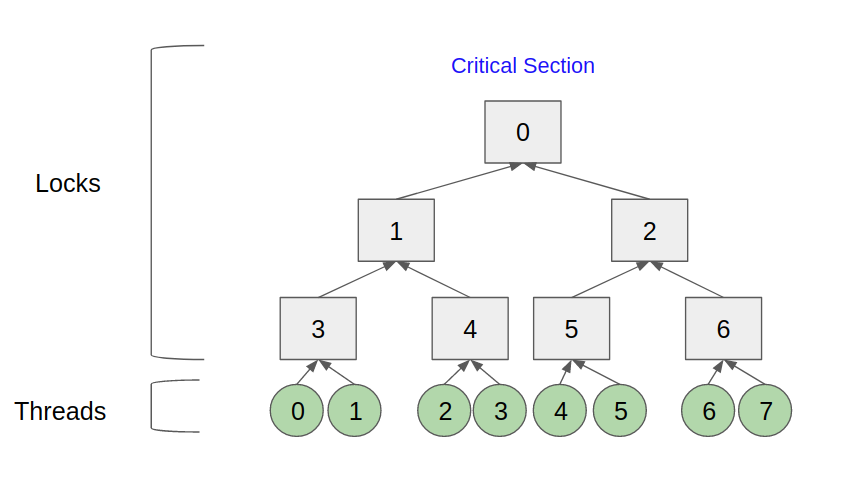
\includegraphics[scale=0.4]{./a.png}
\end{center}
The tree based lock works as seen above requires a thread to aquire all locks (Peterson Lock) on a path from the leaf to the root of a binary tree. The thread which has aquired the root lock can enter the critical section.
Some points regarding the design of the peterson tree based lock are:
\begin{itemize}
\item The tree for \texttt{n} threads would require \texttt{n-1} locks i.e. \texttt{n-1} total nodes ($\because \texttt{n \;threads} \implies \texttt{n/2\; leaf\;nodes}$).
\item Each thread needs to be mapped to one of the leaf nodes. We do this by mapping thread $i$ to the leaf node indexed \texttt{n/2 + i/2 - 1}.
\item Each thread first aquires the leaf lock it is assigned and then proceeds to aquire the subsequent parent locks until the root lock is aquired.
\item Each individual lock is a \textbf{Peterson Lock}. Since there are more than two threads which could possibly try to aquire the same Peterson Lock, we need to change the implementation of the wait condition of the peterson lock. We do this in the following way:
\begin{itemize}
\item Instead of having two flag variables, we have an array called flag of length n, which lets us know if the thread is interested in aquiring the lock.
\item Victim can now take any value from \texttt{1 to n}.
\end{itemize}
\item While unlocking the peterson locks we proceed from the root to the leaves. If we went from leaves to root there would exist a condition where three different threads would have the flag value for the same peterson lock as true. This would violate mutual exclusion, since the peterson lock is meant only for two threads.
\item In a tree with height \texttt{>=2}, the unlock function would proceed from top to bottom in this case there exists the possibility that the root lock is unlocked and another thread aquires it before the orignal thread has unlocked all the locks till the leaf. There is nothing wrong with this and mutual exlusion is preserverd, but from the logs it might appear that there exist more than 1 thread in the critical section. This is simply because of the fact that the other thread does not need to wait for the orignal thread to finish it's unlock method to enter the critical section. While this does not appear in the logs I have generated, it is something which is possible, and more so for a larger value of n.
\end{itemize}
\newpage
\section{Results \& Graphs}
\subsection{Average Waiting Time To Aquire Lock Vs Number Of Threads}
\begin{center}
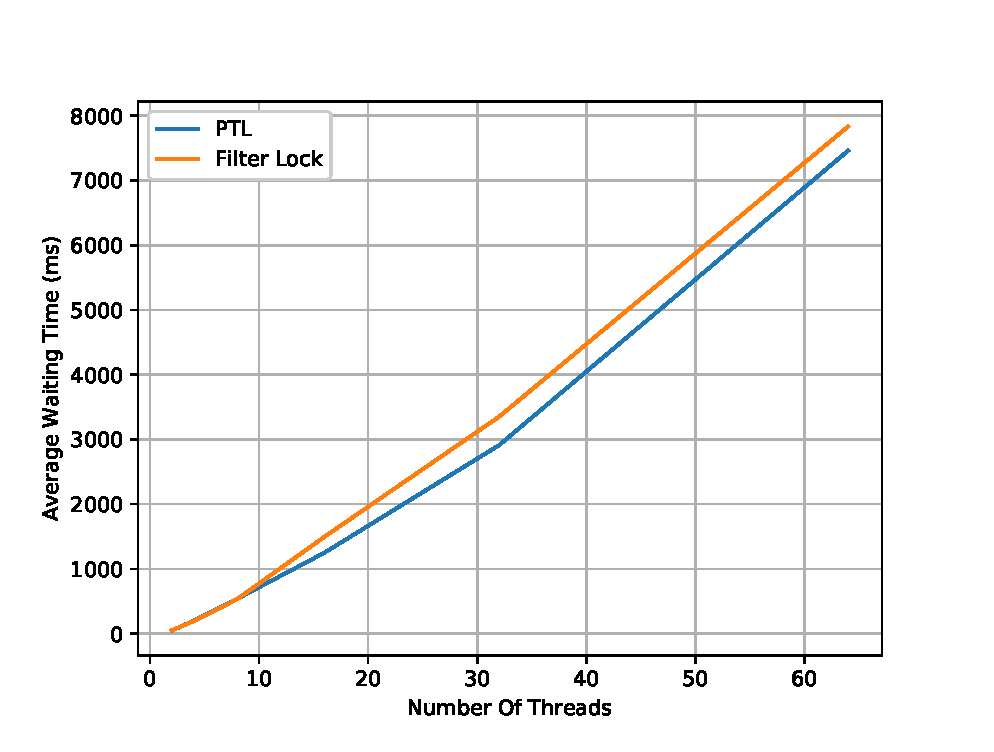
\includegraphics[scale=0.7]{./w.eps}
\end{center}
\subsubsection{Inference}
\begin{itemize}
\item From the curves, it is visible that PTL performs slightly better than filter lock. \item This could be because of the fact that for PTL the thread in the critical section only needs to unlock the root Two Thread Peterson Lock before another thread can enter the critical section. Another minor reason could be that the \texttt{lock} procedure for filter lock needs to access a \texttt{level array} but for the two thread peterson lock it is just a variable, so it would be expected to have faster access times.
\item Other than the minor differences the wait condition for both the algorithms is quite similar, (since the filter lock is just an extension of the Peterson Lock), so we see that asymptotically the curves seem to be converging.
\end{itemize}
\subsection{Average Waiting Time To Unlock Vs Number Of Threads}
\begin{center}
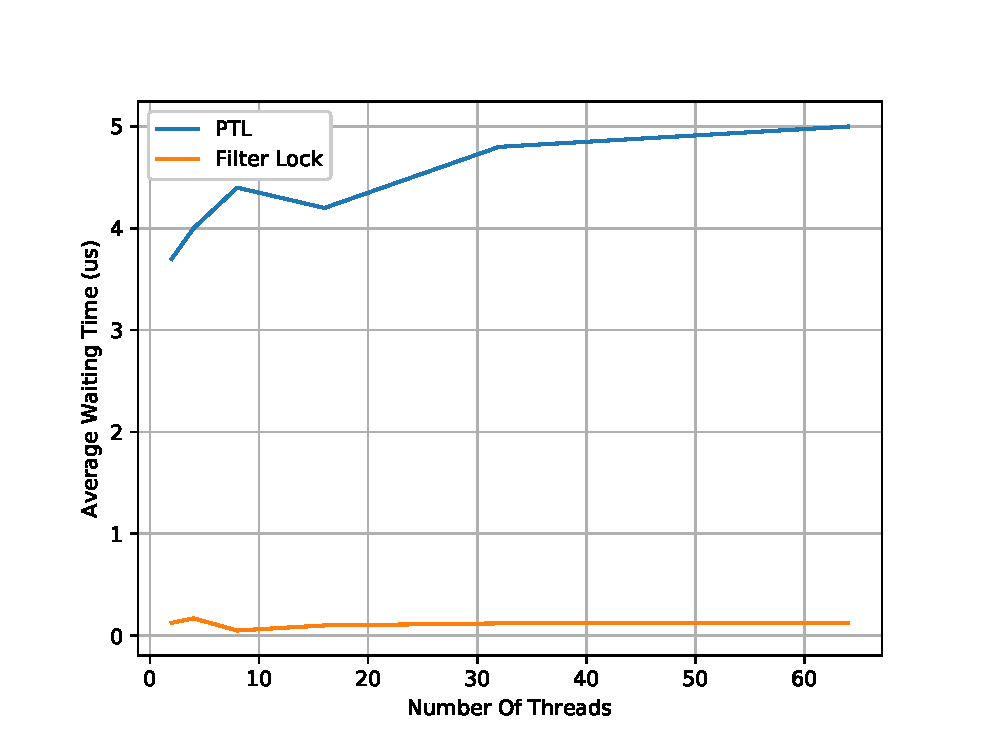
\includegraphics[scale=0.7]{./we.eps}
\end{center}
\subsubsection{Inference}
\begin{itemize}
\item As expected the curve for Filter lock shows that it takes nearly constant and a very small amount of time to unlcok from the Filter lock. This is because the unlock procedure for Filter lock is just a single assignment operation which would take a constant number of cycles on no matter the number of threads that exist.
\item For the Peterson Lock, we do not see much change in the values either. This is because on moving from 2 to 64 threads we are just moving from a single unlock to 5 unlocks, this is because the number of locks to be unlocked increases as the \texttt{log} of the number of threads that are trying to enter the CS. But at the same time it must be noted that the time taken for PTL unlock is greater than the time taken fot the unlock for the Filter lock. This is because Filter lock always has to just assign a single variable, but for PTL, multiple two thread peterson locks need to be unlocked.
\end{itemize}
\end{document}